\documentclass[a4paper, 12pt]{article}
\usepackage[T2A]{fontenc}
\usepackage[left=2cm,right=2cm,top=2cm,bottom=2cm]{geometry}
\usepackage[russian]{babel}
\usepackage{amsfonts,amsmath,amssymb}
\usepackage{mathrsfs}
\usepackage{graphicx}
\usepackage[normalem]{ulem}
\usepackage{wrapfig}
\usepackage{fancyhdr}
\usepackage{floatflt}
\usepackage{python}
\usepackage{indentfirst}
\usepackage{setspace}
\usepackage{scrextend}
\usepackage{listings}
\usepackage{makecell,tabularx}
\usepackage{hyperref}
\usepackage{xcolor}
\usepackage{pdfpages}
\usepackage{tikz}                                                                                                                                                                                                             
\usepackage{graphicx}                                                                                                      
\usepackage{newtxtext}                                                                                                     
\usepackage{float}                                                                                                         
\usepackage{comment}
\usetikzlibrary{calc}   

\newcommand{\rub}{{\rm{Р}\kern-.635em\rule[.5ex]{.52em}{.04em}\kern.11em}}

\definecolor{linkcolor}{HTML}{000000} 
\definecolor{urlcolor}{HTML}{0000FF} 

\hypersetup{pdfstartview=FitH,  linkcolor=linkcolor,urlcolor=urlcolor, colorlinks=true}

\definecolor{grey}{RGB}{40, 40, 40}

\setlength{\headheight}{14.49998pt}
\addtolength{\topmargin}{-2.49998pt}

\renewcommand{\href}[1]{\url{#1}}

\lstdefinestyle{CommentStyle}{language=XML,commentstyle=\color{red},basicstyle=\footnotesize\ttfamily,language={[ANSI]C++},keywordstyle=\bfseries,showstringspaces=false,morekeywords={include, printf},commentstyle={},escapeinside=§§,escapebegin=\begin{russian}\commentfont,escapeend=\end{russian},keywordstyle=\color{blue}\bfseries,morekeywords={align,begin},extendedchars=\true,tabsize=2}
\lstdefinestyle{myLatexStyle}{language=c++,numbers=left, numberstyle=\tiny, stepnumber=1, numbersep=5pt,commentstyle=\color{red},keywordstyle=\color{blue}\bfseries,morekeywords={align,begin},extendedchars=\true,tabsize=2}
\lstdefinestyle{pmyLatexStyle}{language=java,numbers=left, numberstyle=\tiny, stepnumber=1, numbersep=5pt,commentstyle=\color{red},keywordstyle=\color{blue}\bfseries,morekeywords={align,begin},extendedchars=\true,tabsize=2}

\setlength{\parindent}{12,5mm}

\onehalfspacing

\pagestyle{fancy}
\renewcommand{\sectionmark}[1]{\markright{#1}}
\fancyhf{} 
\fancyhead[R]{\bfseries\thepage}
\fancyhead[LO]{\bfseries\rightmark}

\newcommand{\image}[3]{\begin{figure}[h!]\center{\includegraphics[height=#2pt]{#1} }\caption{\textit{#3}}\end{figure}}                                                                                                                
\newenvironment{myfont}{\fontfamily{phv}\selectfont}{\par}                       
\newcommand{\cmd}[1]{\immediate\write18{#1}}
\newcommand{\pf}[1]{\immediate\input{#1}}

%!begin

\begin{document}

\thispagestyle{empty}
\begin{floatingfigure}{5.8cm}
  
\includegraphics[width=5.8cm,height=3.5cm,keepaspectratio]{logo.png}
  \vspace{0cm}
\end{floatingfigure}

\sloppy{
  \scriptsize{
    \line(6,0){0}

    \centering Департамент образования и науки города Москвы

    \centering ГОСУДАРСТВЕННОЕ БЮДЖЕТНОЕ

    \centering ОБЩЕОБРАЗОВАТЕЛЬНОЕ УЧРЕЖДЕНИЕ ГОРОДА

    \centering МОСКВЫ «КУРЧАТОВСКАЯ ШКОЛА»

    \line(6,0){300}

    \centering 123060, Москва, улица Маршала Конева, дом 10.

    \centering \textbf{Тел: (499) 194-10-44, E-mail: kurchat@edu.mos.ru}

    \line(6,0){0}
  }}

\topskip=-200pt
\vspace*{130px}
\begin{Huge}
  \textbf{
    \begin{center}
      Проектная работа по теме:\\«Умное освещение для дома»
    \end{center}
  }
\end{Huge}
\vspace*{5px}
\begin{footnotesize}
  \center {В проекте был продемантсрирован прибор для освещения дома.}
  \vspace*{200px}
  \begin{flushright}
    Выполнил ученик 11 «А» класса\\
    Плютто Андрей Петрович\\
    Руководитель проекта\\
    ---------------------\\
  \end{flushright}
\end{footnotesize}
\begin{normalsize}
  \begin{center}
    Москва\\
    2021-2022 год
  \end{center}
\end{normalsize}
\newpage

\thispagestyle{fancy}
\renewcommand{\sectionmark}[1]{\markright{#1}}
\fancyhf{}
\fancyhead[R]{\bfseries\thepage}
\fancyhead[LO]{\bfseries Оглавление}
\renewcommand{\contentsname}{Оглавление}
\small{\tableofcontents}
\newpage
\pagestyle{fancy}
\renewcommand{\sectionmark}[1]{\markright{#1}}
\fancyhf{}
\fancyhead[R]{\bfseries\thepage}
\fancyhead[LO]{\bfseries\rightmark}

\section{Аннотация}

\newpage
\section{Введение}
\subsection{Актуальность}

%В наши дни тема умного дома набирает популярность и многие люди уже хотят себе
%установить пару-тройку модулей для упрощения повседневных дел. Многие 
%IT-гиганты бьются за место под солнцем, создавая новую или улучшая старую 
%технику до уровня "умного". Под влиянием этого я решил попробовать сделать 
%свой модуль этого же уровня для дополнительного освещения своей комнаты.

%Если говорить более подробно, то я решил сделать подсветку по периметру комнаты 
%с помощью адресной светодиодной ленты. Об актуальности данной идеи и говорить 
%не следует: в секторе освещения для умного дома выбора достаточно мало. Все, 
%что мне удалось найти на просторах интернета: пару устаревших модулей для 
%адресной светодиодной ленты под управлением с пульта и всевозможные виды умных
%ламп, которые, хоть и выглядят красиво, не производят такого эффекта как 
%лента. 

%В интернете я нашел проект, в котором взяли простую белую светодиодную ленту 
%и обклеили ей комнату. Получилось достаточно интересно. Различия между лентами
%я рассмотрел в %!

Тема умного дома набирает популярность в наши дни. Одно из главных направлений 
в этой области -- освещение. Не смотря на то, что это направление является 
очень интересным для покупателей многие компании не могут похвастаться большим
выбором. Я решил использовать адресную светодиодную ленту, так что 
вариантов ее свечения будет очень много. 

\subsection{Проблема}

Освещение комнаты при разном времени суток одинаково, что плохо влияет на 
зрение. Так же динамическое освещение хорошо влияет на настроение и 
психолгическое равновесие.

\subsection{Цель работы}

Создать динамическое освещение, подстраивающееся под уровень света в комнате и 
время суток.

\subsection{Задачи}
\begin{enumerate}
  \item Выяснить для разных естественных освещений какое должно быть искусственное
  \item Создать макет, развести и создать собственный МК для управления лентой
  \item Рассчитать потребление тока лентой 
  \item Создать программу для управление лентой
  \item Соединить МК и ленту
  \item Написать сайт для управления лентой с телефона 
\end{enumerate}

\newpage

\subsection{Предисловие}

В наши дни тема умного дома набирает популярность и многие люди уже хотят себе
установить пару-тройку модулей для упрощения повседневных дел. Многие 
IT-гиганты бьются за место под солнцем, создавая новую или улучшая старую 
технику до уровня "умного". Под влиянием этого я решил попробовать сделать 
свой модуль этого же уровня для дополнительного освещения своей комнаты.

Если говорить более подробно, то я решил сделать подсветку по периметру комнаты 
с помощью адресной светодиодной ленты. Об актуальности данной идеи и говорить 
не следует: в секторе освещения для умного дома выбора достаточно мало. Все, 
что мне удалось найти на просторах интернета: пару устаревших модулей для 
адресной светодиодной ленты под управлением с пульта и всевозможные виды умных
ламп, которые, хоть и выглядят красиво, не производят такого эффекта как 
лента. 

В интернете я нашел проект, в котором взяли простую белую светодиодную ленту 
и обклеили ей комнату. Получилось достаточно интересно.

\image{белая_лента.jpg}{300}{Пример ленты}

Понимая, что могу сделать лучше, я занялся данным проетом и вот что у меня 
получилось.

\newpage

\section{Чем отличаются адресные ленты от обычных?}
В этой части я хочу подробнее рассмотреть и показать слушателю что же такое 
адресная лента. Рассмотрим эволюцию светодиодных лент.

\subsection{Обычная светодиодная лента}
Обычная светодиодная лента представляет собой ленту с напаянными светодиодами и
резисторами, на питание имеет два провода: плюс и минус. Напряжение бывает 
разное: 5 и 12 вольт постоянного тока и 220 переменного. Светит такая лента 
одним цветом, которой зависит от светодиодов. Как можно уже было понять 
функционала в ней крайне мало, но в качестве замены обычной лампы накаливания 
она будет очень кстати, ведь у таких лент самый высокий LUX-коэффициент(самые 
яркие) и при этом они потребляют меньше всего тока.

\image{белая_светодиодная_лента.jpg}{350}{Пример белой ленты}

\newpage

\subsection{RGB светодиодная лента}
На этой ленте стоят RGB светодиоды. Такой светодиод имеет уже 4 выхода, один 
общий 12V (анод), и три минуса (катода) на каждый цвет, т.е. внутри одного 
светодиода находится три светодиода разных цветов. Соответственно такие же 
выходы имеет и лента: 12V, G, R, B. Подавая питание на общий 12V и любой из 
цветов, мы включаем этот цвет. Подадим на все три – получим белый, зелёный и 
красный дадут жёлтый, и так далее. Такие ленты очень распространены и их 
наверняка видел каждый. Однако для динамической подсветки в комнате они вряд ли
подойдут тк за раз они могут светить лишь одним светом.

\image{RGB_светодиодная_лента.jpg}{450}{Пример RGB ленты}

\newpage

\subsection{Адресная светодиодная лента}
Адресная светодиодная лента, вершина эволюции лент. Представляет собой ленту из
адресных диодов, один такой светодиод состоит из RGB светодиода и контроллера.
Благодаря такой начинке у нас есть возможность управлять цветом любого 
светодиода в ленте и создавать потрясающие эффекты. Адресная лента может иметь 
3-4 контакта для подключения, два из них всегда питание (5V и GND например), и 
остальные (один или два) – логические, для управления.

\image{Адресная_светодиодная_лента.jpg}{230}{Пример адресной ленты}

Лента “умная” и управляется по специальному цифровому протоколу. Это означает, 
что если просто воткнуть в ленту питание не произойдет ровным счётом ничего, то
есть проверить ленту без управляющего контроллера нельзя. Если вы потрогаете 
цифровой вход ленты, то скорее всего несколько светодиодов загорятся 
случайными цветами, потому что вы вносите случайные помехи, которые 
воспринимаются контроллерами диодов как команды. 

Думаю теперь вам стал понятен мой выбор в пользу светодиодной адресной ленты.

\newpage

\section{Как выбрать блок питания?}

Для начала разберемся что такое блок питания.
Блок питания - это источник напряжения(трансформатор), который преобразует 220В
переменного тока в необходимое значение постоянного тока. 

\image{блок_питания.jpg}{150}{Пример блока питания}

Чтобы подобрать блок питания к выбранной светодиодной ленте нужно обратить 
внимание на следующие факторы:

\begin{enumerate}
\item Рабочее напряжение светодиодной ленты.
\item Суммарная мощность светодиодной ленты.
\item Необходимость защиты корпуса блока питания от воды и пыли.
\itemГабаритные размеры блока питания.
\end{enumerate}

Рассмотрим подробнее каждый фактор.

\subsection{Рабочее напряжение (U)}

Рабочее напряжение светодиодной ленты может быть 5V, 12V, 24V, 36V. 
Соответственно оно должно соответствовать выходному напряжению блока питания. 

\begin{table}[H]
    \begin{center}
    \begin{tabular}{|c|c|c|c|}
        \hline
        Чип&	Напряжение	\\
        \hline
        WS2811&	12-24V\\
        WS2812&	5V\\
        WS2813&	5V\\
        WS2815&	12V\\
        WS2818&	12/24V\\
        \hline
    \end{tabular}
\end{center}
\centering{Таблица 1:Напряжение адресных лент в зависимости от чипов}
\end{table}
Так как я решил использовать адресную светодиодную ленту WS2812 то нужное мне
напряжение 5V. Для данного проекта рекомендую использовать именно тот чип 
т.к. логика чипа, о котором я буду говорить ранее именно 5V.

\subsection{Мощность светодиодной ленты (P)}

Подбор блока питания по мощности осуществляется по следующему принципу: 
мощность должна быть равна суммарной мощности светодиодов ленты.

Для вычисления мощности используют формулу 

$$P=UI$$

Где U=5V, сила тока (I) равна сумме силы необходимой для каждого светодиода 
ленты $I_1$=0.36мА. Таким образом взяв длину ленты(l) и кол-во светодиодов на 
метр(n) мы получим формулу

$$I=I_1ln \Rightarrow P=UI_1ln$$

Я понимаю что многим будет достаточно сложно рассчитать необходимую мощность, 
так что я создал небольшой калькулятор, в который забив необходимые параметры 
ленты можно получить необходимую силу тока или мощность для БП. Если вы не 
найдете блока с такими параметрами берите с запасом, ленте от этого точно хуже 
не будет. Калькулятор можно найти на странице 
https://pluttan.github.io/calc\_for\_KelBilight/ или на странице ESP, о которой
будет рассказано позже. 

Так же для некоторых стандартов я расщитал мощность сам.

\begin{table}[H]
    \begin{center}
    \begin{tabular}{|c|c|c|c|}
    \hline
    Кол-во светодиодов & Длина ленты(l(м)) & Сила тока (I(А))& Мощность тока(P(Вт)) \\
    на метр(n)&&&\\
    \hline
     30 &  5 &  5 &  26\\
     30 & 10 & 10 &  53\\
     30 & 15 & 16 &  81\\
     30 & 20 & 21 & 107\\
     \hline
     60 &  5 & 10 &  53\\
     60 & 10 & 21 & 107\\
     60 & 15 & 32 & 162\\
     60 & 20 & 43 & 215\\
     \hline
    120 &  5 & 21 & 107\\
    120 & 10 & 43 & 215\\
    120 & 15 & 64 & 324\\
    120 & 20 & 86 & 431\\
    \hline
    \end{tabular}
    \end{center}
    \centering{Таблица 2:Мощности токов}
\end{table}

\subsection{Степень защиты корпуса блока питания от проникновения жидкости и пыли (класс защиты IP)}

При выборе блока питания следует учитывать условия, в которых он будет 
находиться, если это обычное сухое жилое помещение, то подойдет блок питания в 
защитном кожухе с IP20 (защита от проникновения твердых предметов 12,5 мм, 
защиты от влаги нет).

Зачастую в блоках питания мощность более 250Вт в исполнении "Защитный кожух" 
IP20-IP40 используется активное охлаждение в виде кулера(вентилятора). Если Вы 
планируете рассматривать данные блоки питания, необходимо выбрать конструктив, 
когда кулер расположен перпендикулярно элементам платы в изделии, следовательно
обдув воздуха будет более равномерный (воздух идет вдоль платы), и элементы 
будут меньше греться. На неудачных моделях вентиляторы расположены над платой 
и обдув платы источника напряжения происходит неравномерно.

\image{ip_блоки_питания.png}{130}{Блоки со стандартом ip20, ip40, ip60}

Блоки питания и комплектующие для лент рекомендуется устанавливать в щитовые.

\subsection{Габаритные размеры}

Также следует обращать внимание на габаритные размеры блоков, в зависимости от 
того, куда Вы хотите его установить, мощные блоки питания могут достигать 
достаточно больших размеров, и спрятать такие будет затруднительно, к тому же 
часто они имеют вентилятор. Поэтому если требуется подключить длинный участок 
ленты, то можно пересмотреть схему подключения ленты и использовать несколько 
меньших по мощности блоков.

Также при выборе места установки следует учитывать то, что чем мощнее блок 
питания, тем больше он нагревается, поэтому рекомендуется обеспечивать 
достаточно места для теплоотвода, чтобы блок не перегревался.

\begin{table}[H]
    \begin{center}
    \begin{tabular}{|c|c|}
    \hline
    Мощность(при 5В) & Размеры \\
    \hline
    10Вт  &  $70  \times  30 \times 40$ \\
    25Вт  &  $85  \times  58 \times 35$ \\
    30Вт  &  $85  \times  58 \times 35$ \\
    40Вт  &  $85  \times  58 \times 35$ \\
    50Вт  &  $160 \times  98 \times 42$ \\
    75Вт  &  $160 \times  98 \times 42$ \\
    100Вт &  $198 \times  98 \times 42$ \\
    150Вт &  $198 \times  98 \times 42$ \\
    200Вт &  $198 \times 110 \times 50$ \\
    250Вт &  $198 \times 110 \times 50$ \\
    \hline
    \end{tabular}
    \end{center}
    \centering{Таблица 3:Габаритные размеры}
\end{table}

\section{Как соединить куски ленты?}
Если каждый кусок ленты соединить просто по пинам выхода и входа, то лента 
может не загореться или загореться неполностью, ведь напряжение может просесть.
В целях избежать просадки напряжения производители делают ленты длиной не 
более 5м. Таким образом мы получаем, что каждые 5м нужно ставить новый блок 
питания. Это давольно затратно, так что был придуман другой способ: просто 
провести провода с большим сечением параллельно ленте к другой. Насколько 
сечение должно быть большое? Можно вычислить по формуле 

$$S=\frac{0.018lI}{U}$$

Где l -- длина провода, I -- сила тока необходимая для питания второго куска ленты, 
U -- напряжение. Но если немного подумать то при U=5В просадки напряжения совсем 
не будет т.е. провод не будет обладать сопротивлением, поэтому за напряжение а 
данных расчётах берут минимально возможное + запас. Как указано в документации 
к ленте минимально возможное напряжение 4.5В. Запас принято брать 0.1-0.3В.

\image{схема_для_кусков.jpg}{70}{Схема соединения кусков ленты}

Обратите внимание: в моем калькуляторе не предусмотрен расчёт площади 
поперечного сечения, но предусмотрено предупреждение о том, что каждый кусок 
ленты в 5м нужно соединять отдельными проводами.

\newpage

\section{Микроконтроллер}

В этой части мы поговорим о микроконтроллере, который будет управлять лентой.

Думаю многие могли подумать на счет популярного микроконтроллера на базе чипов 
AltMega — Arduino. Свои работы я начинал именно на нем. Многое предстояло 
сделать, так что я решил сразу начать с программирования, а с “железом“ я решил
разобраться позже.

\image{arduino.jpg}{120}{Ардуино UNO}

В процессе программирования я попробовал многие способы управления светодиодной 
лентой начиная с библиотек закачивая собственным бинарным кодом. Далее я 
расскажу об этом. Сейчас я бы хотел обратить ваше внимание на то, что 
оперативная память в микроконтроллере очень маленькая. Некоторые могут отметить 
что есть новые серии Arduino Nano — RP2040, но настолько мощный микроконтроллер 
будет жаль использовать в данной ситуации. 

Долго размышляя, я пришел к выводу, что единственный выход сделать собственный 
контроллер с дополнительной памятью SRAM на базе той же AltMega 328, что стоит 
в Arduino Nano 3.0.

\image{sram&altmega.jpg}{120}{Память SRAM и AltMega 328}

Но не только вывод для ленты нужен этому микроконтроллеру но и пару сенсоров 
для того, чтобы действительно назвать его умным.

Посмотрим на примерный план всего того, что нужно:
\begin{enumerate}
\item Датчик цвета
\item Радио модуль
\item WiFi модуль
\end{enumerate}
С этим мы разберемся по порядку, но для начала предлагаю разобраться с 
“нуждами“ самого процессора.

\newpage

\subsection{Процессор}
\subsubsection{Тактирование}
Я не очень хочу нагружать свой реферат излишней информацией, но желаю донести 
хотя бы основы тактирования процессоров до читателя.

Что же такое тактирование? Для начала следует отметить, что любая команда 
выполняется процессором в таком порядке:

\begin{itemize}
  \item Получить из памяти команду
  \item Получить требуемые для выполнения команды данные
  \item Выполнить команду и сохранить результат
  \item Перейти к выполнению следующей команды
\end{itemize}

После выполнения последней команды процессор перейдет к выполнению первой в 
цикле(loop). 

Эти 4 этапа, будут соответствовать 4 состояниям процессора. Этапы называют 
тактами процессора. Все четыре этапа, вместе взятые, образуют машинный цикл. 
Таким образом, машинный цикл состоит из четырех тактов. Иногда это называют 
фазами работы процессора. Теперь нам надо сформировать сигналы управляющие 
работой узлов процессора и соответствующие этим 4 фазам.

Еще в прошлом веки инженеры договорились, что за логическую единицу и 
логический ноль поданных на специальные “ноги“ процессор выполнит 1 такт. 

\image{tact.png}{300}{Схема тактов(сверху подаваемые сигналы, далее -- такты.)}

Это означает что если мы соединим XTAL1 и XTAL2, а затем разъединим то это 
будет считаться за 1 такт. Следует обратить ваше внимание, что если мы сделаем 
это слишком быстро, то процессор просто не успеет выполнить такт за отведенное 
ему время и скорее всего перегорит. Ну а если мы сделаем это слишком медленно, 
то процессор перейдет  на внутреннее тактирование и сбавит скорость выполнение 
команд с максимальной.

О внутреннем тактировании можно почитать в документации самого процессора, но 
очень часто его занижают в целях уменьшения теплоотдачи самого процессора. Так 
же в современных компьютерных процессорах можно изменять скорость тактов 
программно, но делать это крайне не рекомендуется опять же из-за 
неконтролируемой теплоотдачи.

Скорость тактов можно вычислить по тактовой частоте -- величине, по которой 
характеризуются кристаллы тактирования. Далее в тему я углубляться не буду и 
перейду к практическому применению.

Из документации ALTMega 328 мы получаем график

\image{график_тактирования.png}{150}{График тактирования}

Так как мы питаем контроллер от 5В, то можно брать как 8MHz, так и 16MHz. Для 
более быстрой работы я конечно выбрал 16MHz. Вот схема установки кристалла.

Как можно увидеть каждой из ног кристалла я кроме “ног“ XTAL1 и XTAL2 (“ног 
тактирования“) я подсоединил конденсаторы на 22pF для сглаживания сигнала 
(более быстрого падения частоты до логического нуля в связи с зарядом 
конденсатора).

\image{Схема_тактирования.png}{100}{Схема кристалла тактирования}

\newpage

\subsubsection{Напряжение, перезагрузка и программатор}

Для стабилизации напряжения к GND и 5V(VCC) я подключил конденсатор емкостью 
100nF(0.1uF).

\image{Стабилизация_напряжения.png}{80}{Схема стабилизации напряжения}

Для подачи напряжения я вывел 2 контакта.

\image{Вывод_пинов.png}{80}{Схема вывода пинов}

Вывел 6 контактов под программатор USB ASP.

\image{Схема_переходника_под_программатор.png}{100}{Схема кнопки перезагрузки}

Для перезагрузки я вывел кнопку RST и подал логическую единицу на одноименный 
пин.

\image{схема_RST.png}{130}{Схема кнопки перезагрузки}

\newpage


\subsection{WiFi модуль}

В качестве WiFi модуля я решил использовать младшую версию ESP8266. Перед тем 
как перейти к разводке самой платы предлагаю посмотреть немного документации к 
ней:

\image{документация_к_esp.png}{300}{Отрывок из документации к ESP8266}

\subsubsection{Плата понижения напряжения}

Здесь видно что сама плата питается от 3-3.3V. Поэтому нужно сделать  
дополнительную плату понижения напряжения.

Делал я ее на базе AMS1117. Такая же соединяет выход 3.3V и 5V на оригинальной 
Arduino.

\image{Схема_понижения_напряжения.png}{100}{Схема платы понижения напряжения}

Два конденсатора слева и справа для уменьшения помех в цепи и для 
того, чтобы не перегружать AMS.

\subsubsection{Кнопки PROG и ESP\_RST}
Кнопка PROG зажимается при записи программы в ALTMega и предназначена для 
программирования ESP. При зажатии ее мы подаем логический ноль в пин IO0 тем 
самым переводя плату в режим программирования.

\image{Схема_кнопка_prog.png}{150}{Схема кнопки prog}

Так же для программирования ESP необходимо ввести в цикл перезагрузки ALTMega. 
Для этого я дополнительно вывел контакты RST и GND.

\image{Схема_вывода_rst.png}{100}{Схема выводов RST}

Кнопка ESP\_RST предназначена для перезагрузки платы ESP и не влияет на ALTMega. 

\image{Схема_кнопка_esp_rst.png}{150}{Схема кнопки ESP\_RST}

\newpage

\subsubsection{Разводка ESP8266-01}
Сама плата разведена очень легко TX-TX RX-RX так как RX имеет логику в 5V, то 
он подключен через резисторы. GND-GND, VCC-3.3V. Остальные с подключены по 
логической единице. 

\image{Схема_ESP.png}{100}{Схема ESP}

\subsection{Радио модуль}
Так как я решил использовать уже готовый китайский модуль, то я просто вывел 
контакты в соответствии с контактами модуля.

\image{Схема_радиомодуля.png}{100}{Схема радиомодуля}

\subsection{Плата расширения(SRAM)}
Подключил к аналоговым пинам ALTMega и подал на HOLD логическую единицу, т.к. 
модуль должен постоянно обрабатывать весь массив цветов в ленте.

\image{Схема_SRAM.png}{100}{Схема SRAM}

\subsection{Вывод для ленты}
Тут я не стал делать дополнительные предохранители и просто поставил контакт 
от процессора, но если не будет хватать питания лента сможет питаться от 
процессора и неправильно будет считывать цвета, если это произойдет то будет 
необходимо припаять к этому контакту дополнительно резистор на 220Ом.

\image{Схема_вывода_ленты.png}{100}{Схема вывода ленты}

Всю схему целиком можно увидеть в приложении 1. Разводка выполнена в 2 слоя, 
оба слоя можно увидеть в приложениях 2 и 3.Так же я сделал корпус для данного 
микроконтроллера в Fusion 360. Корпус можно посмотреть в приложении 4, а крышку 
от него в прижожении 5.

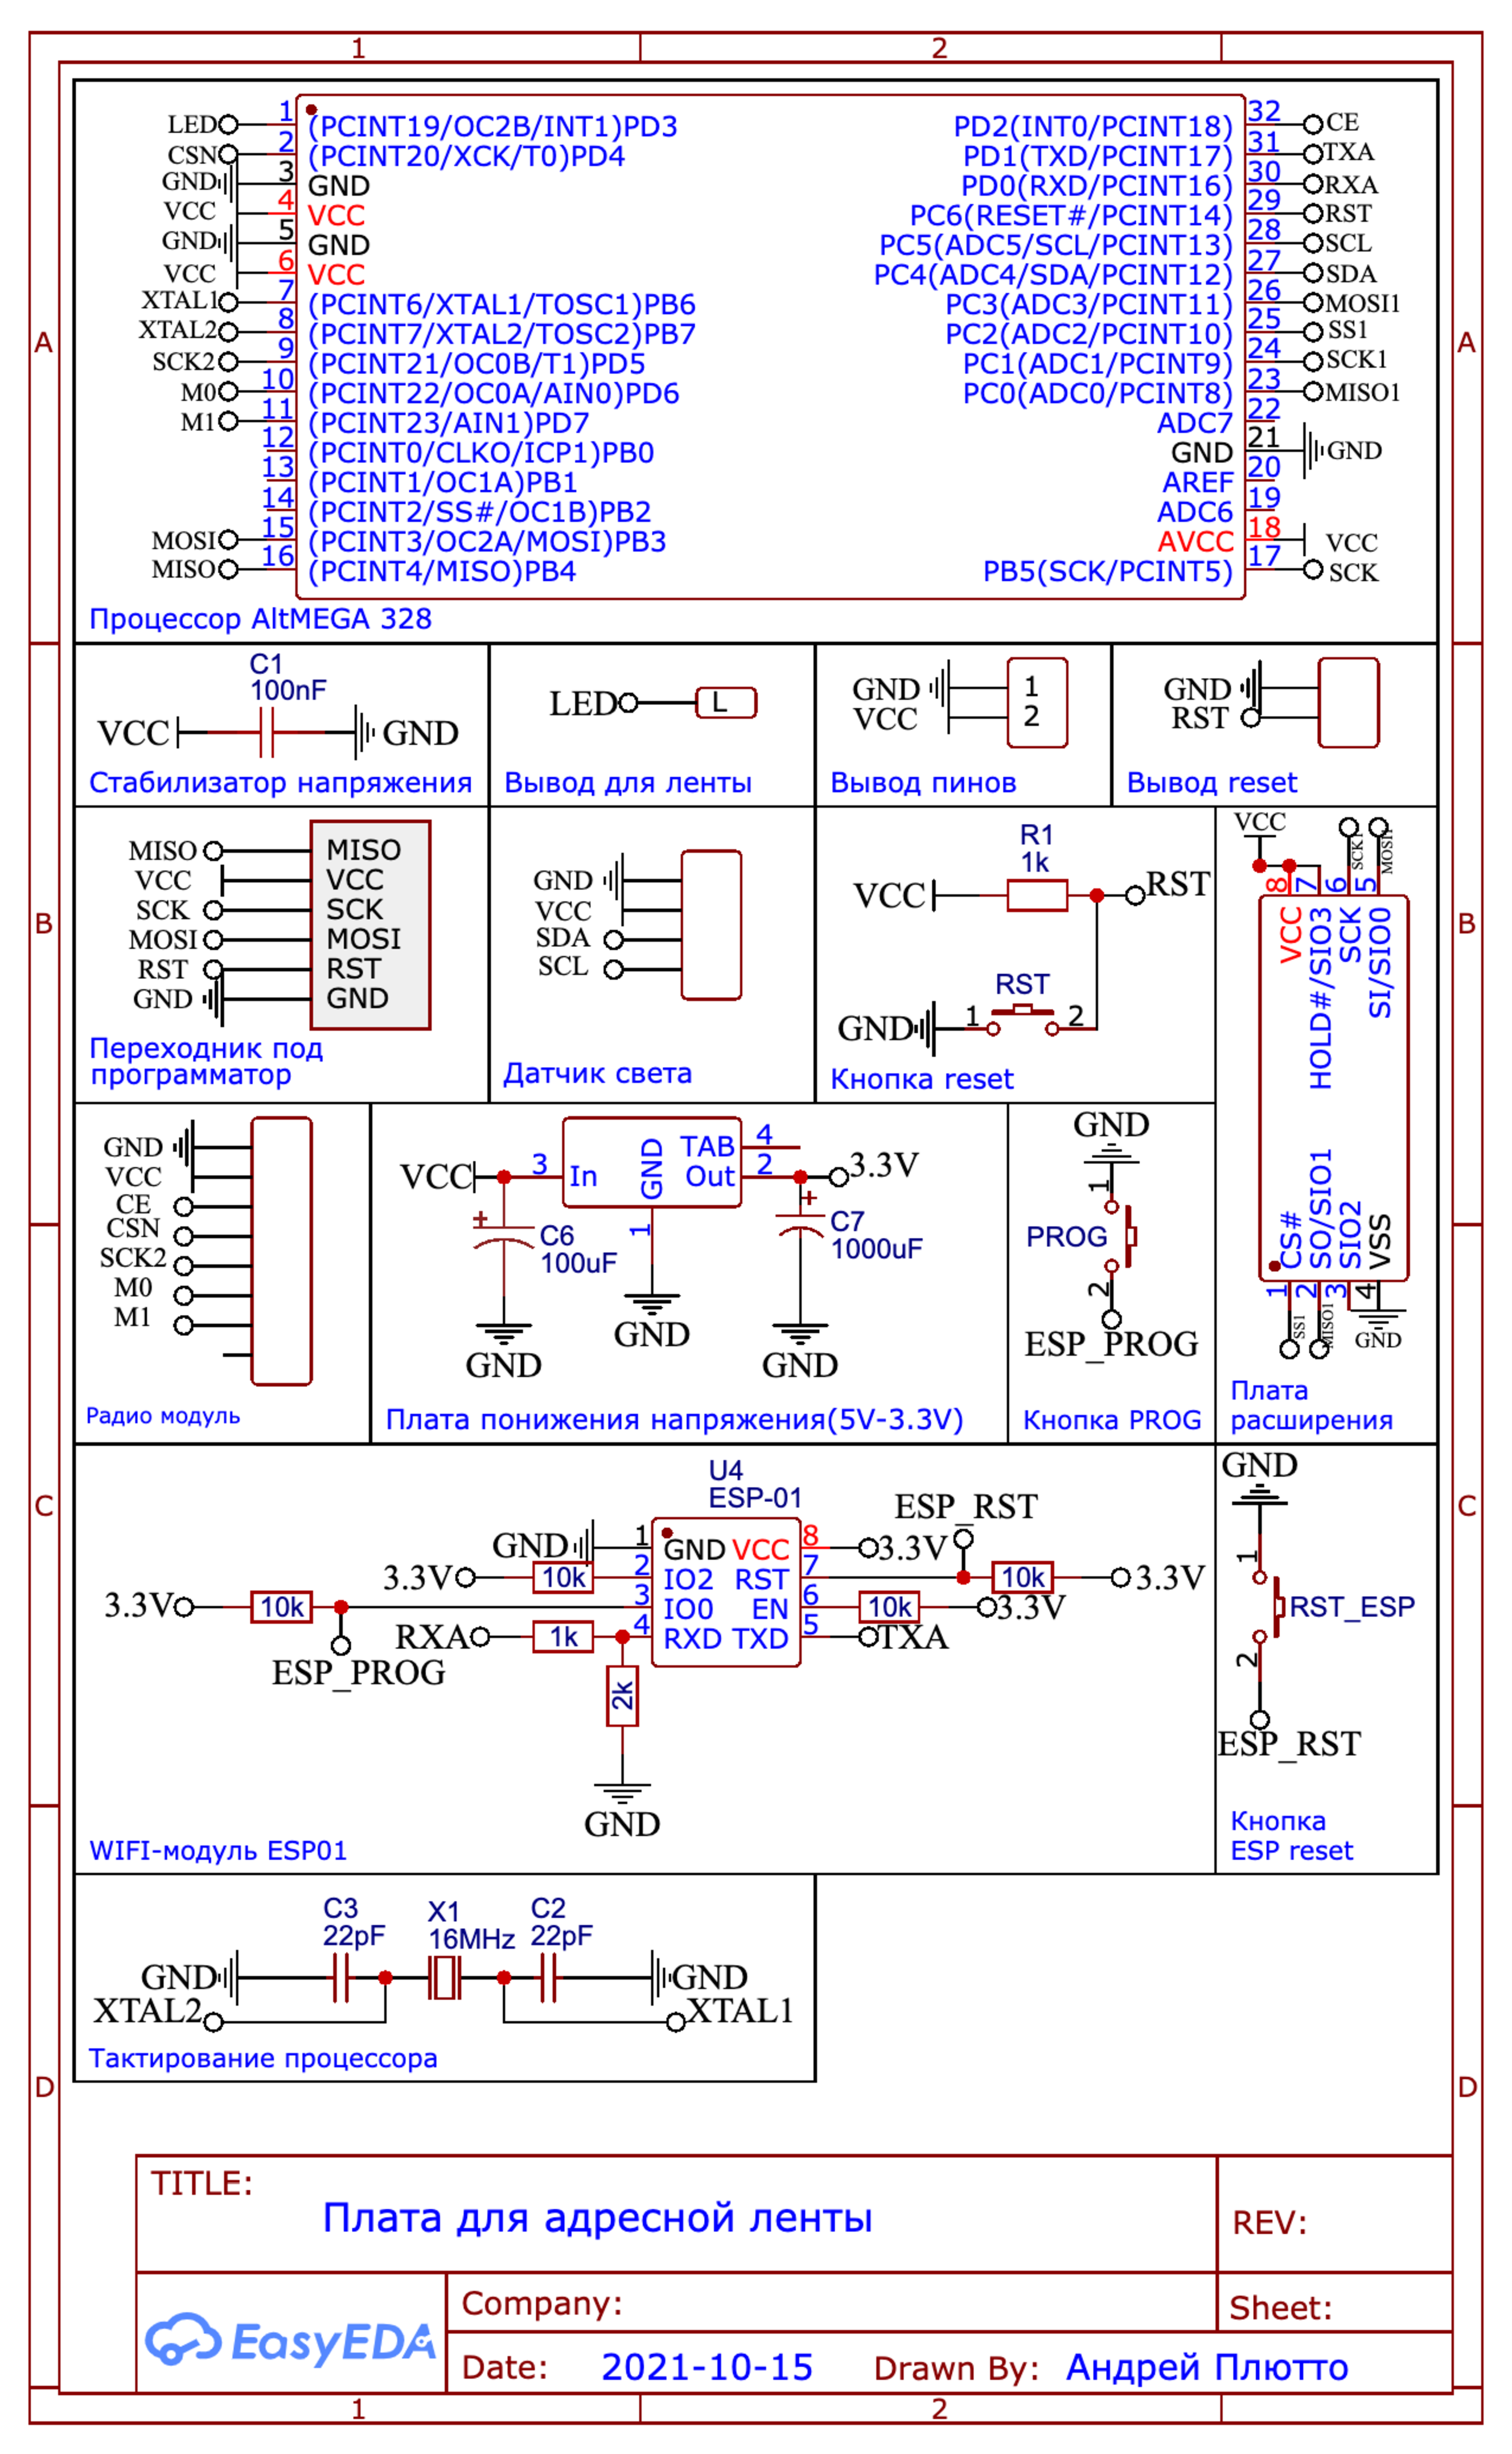
\includepdf[delta=0 12]{/Users/pluttan/Desktop/дом/KelVin/doks/KelBilight/conf/Приложение_1.pdf}\centering{Приложение 1: Схема микроконтроллера}\newpage


\end{document}